\setlength{\footskip}{8mm}

\chapter{Methodology}
\label{ch:methodology}

\textit{Court cases can be structured as legal arguments between the plantiffs, defendants and the Court. The arguments that stand in the end can be said to be the winning argument.
In this study we will:  1.) choose legal disputes related to marine insurance where the issue is with proximate cause  2.) identify the rules, facts and arguments in the case, and structure the case to fit into the Argumentation Framework. 3.) Structure the case to fit into the Argumentation Framework. 4.) Evalute the arguments in PROLOG.}

\section{Flota Mercante Dominicana v American Manufactureres Mutual Insurance Company}
% FACTS -----------------------------------------------------------------------------------

\newcommand{\factOne}{Plaintiff was the owner of the SS SANTO DOMINGO which burned and sank in the harbor of Santo Domingo, Dominican Republic, following shelling by members of the U.S. Armed Forces on May 4 and 5, 1965.}

\newcommand{\factTwo}{On April 24, 1965, the vessel cleared New York bound for Santo Domingo. The same day the news of the uprising in the Dominican Republic reached the ship}

\newcommand{\factThree}{According to the testimony of the ship’s captain, the broadcasts were greeted with nervous excitement by the crew. There was considerable drinking of alcoholic beverages, much hanging about the radio operator’s quarters and a general loosening of the crew’s discipline. A couple of days out of Santo Domingo, a deputation led by the first cook waited on the captain and persuaded him to permit transmission of a message sympathetic to the new constitution.}

\newcommand{\factFour}{On approaching the harbor of Santo Domingo, the captain held a meeting of the officers to discuss the question of putting into the harbor. The captain’s orders on leaving New York were to proceed to Santo Domingo, and he had received no change in those orders. He had had previous experience with navigating during revolutions, coups and uprisings in the Dominican Republic, none of which had resulted in seriously damaging consequences. Moreover, the atmosphere on ship was tense (the captain slept with a hand gun beneath his pillow), and the crew had made it clear by their behavior that they wished to enter Santo Domingo. In these circumstances, it was decided to enter the port.}

\newcommand{\factFive}{The ship went into Santo Domingo on April 29 and tied up in the Ozama River about 200 meters from a fort then in the hands of National Police loyal to the regime which had been in power when the troubles broke out. The captain gave both crew and passengers instructions to remain on the ship while he went ashore to investigate the situation. The captain attempted to get in touch with the owners of the vessel and to ascertain the conditions in the town. He quickly discovered that he was in the center of a battlefield and he was unable to return to the ship. }

\newcommand{\factSix}{It is unclear what the crew and passengers did to care for themselves, but the succeeding events suggest that within the next several hours each sought safety or excitement with the army of his choice. }

\newcommand{\factSeven}{The next day the forces in the fort next to the ship, roughly 1,000 National Police, came under heavy pressure from the new constitutionalists, who appear to have taken command of those parts of the city lying on the side of the fort away from the river. Further, the National Police in the fort had had nothing to eat for three days. An evacuation of the fort was ordered. Four to five hundred of the retreating police went aboard the SS SANTO DOMINGO, which apparently was empty at that time, seeking refuge, food and modes of escape from the opposing forces. An unsuccessful attempt was made to release the ship from her moorings (by firing machine gun volleys at the cables), a couple of the lifeboats were used to ferry the troops across the Ozama River and whatever food and clothes were found aboard were taken. Within the space of several hours, the ship was abandoned by the retreating police forces.}

\newcommand{\factEight}{The vessel was then rapidly occupied by the rebel forces. The new occupants of the ship used it to direct fire at elements of the 82nd Airborne Division which had been sent to the Dominican Republic under the executive order of President Johnson to protect American nationals and had taken up positions on the other side of the Ozama River. There were exchanges between the American and Dominican rebel forces which came to an end when the Americans resorted to the use of 106 mm explosive shells. Hits by two of these shells on May 4th and 5th caused the ship to burn and sink so that she became a constructive total loss.}
%\FACTS -----------------------------------------------------------------------------------

\subsection{Introduction}

The dispute follows a sequence of events that led to the sinking of the ship SS SANTO DOMINGO during an uprising in Dominican Republic.
The main issues that led to the dispute are disagreement on the proximate cause and ambiguity in in insurance contract.

% TODO: What is task of the ship?

\subsubsection{The Insurance Policies}

The insurance policies define the circumstances and exemptions under which the insured can make a claim to the insurer for a loss. If the loss falls under these valid circumstances, the insurer must pay the insured for the loss.

\textbf{The War Risk Policy}

The war risk policy protects the insured from losses that occur due to the risks of war.

It contains 2 exemptions that are relevant to this case.

1. If loss is due to capture, seizure, arrest, restraint, detainment, preemption, confiscation or requisition by the country in which the vessel is owned or registered is not covered.

2. If loss occurs after requisition by the country in which the vessel is owned or registered, it is not covered.

\textbf{The Hull Policy}

The hull policy protects the insured from loss that occurs due to damage to the ship.

It contains one exemption relevant to this case: The free of capture and seizure clause, which effectively removes the war risk coverage from the hull policy.  

\subsubsection{Proximate Cause}

Proximate cause is concerned with how the actual loss or damage happened to the insured party and whether it is a result of an insured peril. It looks for what is the reason behind the loss, is that is an insured peril or not.

The fundamental principle underlying every contract of marine peril insured against, or as the legal maxim states: "causea proxima non remota spectatur" -- the proximate and not the remote cause must be looked to. \cite{marineInsuranceAct55}

\subsubsection{Finding the proximate cause}

In order to assign liability, the Court must find the proximate cause of the loss of the ship and then
determine whether that cause fell within any of the exceptions of the policy involved.

In order to achieve some degree of certainty in assigning liability,
admiralty courts have relied on the \textit{maxim of causa próxima non remota spectatur}
and when interpreting  proximate cause in marine insurance cases, the courts have
tended to apply it stringently.

Thus, searching backward from the
caused event for the proximate cause, the courts have sought out the first cause
from which the event flows in a natural, almost mechanical and inevitable manner;
what has been called “the real efficient cause of the loss.”

This canon of stringent construction is helpful in assigning
liability and in providing a measure of predictability by which shipowners and
underwriters can measure risk and set rates, but ultimately the courts must use common sense in deciding which strand in the net of causation is the proximate cause of the accident.

\subsubsection{Resolving ambiguous terms in the policy}

Courts follow the \textit{contra proferentem canon} to resolve ambiguous terms in a contract. According to this, the court should construe the ambiguities of a contract against the writer of the contract. 

\subsubsection{Events that led to the loss}

E1: SS SANTO DOMINGO set sail from New York to Santo Domingo, The same day as news of an uprising there.

E2: News of rebellion led to considerable drinking and loosening of the crew's discipline. 

E3: A deputation led by the first cook waited on the captain and persuaded him to permit transmission of a message sympathetic to the new constitution

E4: On approaching the harbor, the captain held a meeting of the officers to discuss the question of putting into the harbor, where it was decided to enter the port.

E5: The ship was docked 200 meters from a fort held by the National Police (loyal to the regime).

E6: The captain left the ship to investigate the situation, ordering the crew and passengers to remain on the ship. The captain soon discovered he was in the middle of a battlefield and was unable to return to the ship. 

E7: Within several hours the crew and passengers deserted the ship.

E8: National Police (numbering ~1000) occupying up in the fort were ordered to evacuate it.  

E9: 400-500 of the retreating police went aboard the empty ship seeking refuge, supplies and modes of escape from the opposing forces. After unsuccessfully attempting to release the ship from it's moorings, the police abandoned the ship with whatever food and supplies that were found along with some lifeboats.

E10: The vessel was soon occupied by rebel forces, who used it to direct fire at American forces. In the resulting exchange of fire, the ship was sunk, resulting in it's total constructive loss.

% \begin{figure}[H]
%   \centering
%   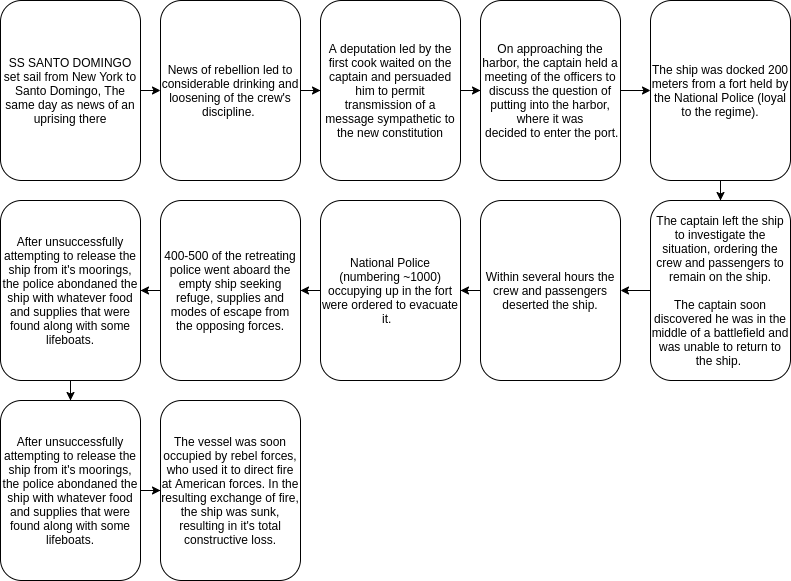
\includegraphics[width=5in]{figures/story.png}https://www.overleaf.com/project/5eb80d515c4db400012d0f3e
%   \caption[Timeline of events]{\small timeline of the events that led to the sinking of the ship.}
%   \label{fig:story}
% \end{figure}

\subsection{Rules}

\subsubsection{Rule1: War Risk Policy} 

    \textbf{If:} loss is due to risks of war.
    
    \textbf{Then:} The loss is covered by the war risk policy.

\subsubsection{Rule2-a: War Risk Policy - Exemption 1}

    \textbf{If:} loss is due to capture, seizure, arrest, restraint, detainment, preemption, confiscation or requisition country in which the vessel is owned or registered
    
    \textbf{Then:} the loss is NOT covered by the war risk policy.
    
    From the case text:
    
    \textit{
    ...An earlier clause excepts
    from the coverage of the war risk policy “any claim arising from capture, seizure,
    arrest, restraint, detainment, preemption, confiscation or requisition” by the
    country in which the vessel is owned or registered...
    }

\subsubsection{Rule2-b: War Risk Policy - Exemption 2}

    \textbf{If:} loss occurs after requisition by country in which the vessel is owned or registered.
    
    \textbf{Then:} the loss is NOT covered by the war risk policy.
    
\subsubsection{Rule3: Hull Policy}

    % (todo: find literature)
    
    \textbf{If:} loss is due to damage to the body of the ship. 
    
    \textbf{Then:} The loss is covered by the Hull Policy.

\subsubsection{ Rule4: Hull Policy - Excemption: FC \& S}

    % (todo: find literature)
    
    \textbf{If:} loss is due to nuclear weapons, mines, torpedoes, war (including civil war), piracy, and confiscation or nationalization of property.
    
    \textbf{Then:} the loss is NOT covered by the hull policy.


\subsubsection{Rule5: causa próxima non remota spectatur}

Whenever the cause of any act or circumstance is need to be understood the immediate cause needs to be looked at and not the remote cause.

Case laws used here:

Standard Oil Co. of New Jersey v. United States, 340 U.S. 54, 58, 71 S. Ct. 135, 95 L.Ed. 68 (1950),

Lanasa Fruit Steamship \& Importing Co. v. Universal Ins. Co., 302 U.S. 556, 562, 58 S.Ct. 371, 82 L.Ed. 422 (1938).

Arnould on Marine Insurance (13th ed., Chorley, 1950) § 785

Lanasa Fruit, supra, at 572, 58 S. Ct. at 378.

% \subsubsection{To define requisition}  

% There are a few suggestive sources for
% the interpretation of this word. Oppenheim describes requisition as “the name for
% the demand for the supply of all kinds of articles necessary for an army.” 2
% Oppenheim’s International Law (7th ed., Lauterpacht, 1955) § 147.

% Article LII of the Second Hague Conventions signed by both the U.S. and the Dominican Republic
% lays out rules for the making of requisitions: that they shall be made only by the
% commander in the locality and shall be paid for as far as possible in cash or a receipt
% given. 2 Treaties, Conventions, International Acts, Protocols and Agreements
% between the U.S. and Other Powers 1776-1909, 2220, 2289

\subsubsection{Rule6: No extended litigation when marine and war risk are with same insurer}

From Gilmore \& Black, The Law of Admiralty, \§ 2- 11 (1957):

\textit{Where possible, the sound plan is for the assured to place his marine and war risks
with the same underwriter, so that the question which sort of risk has caused his
loss can have no practical importance.}

\subsubsection{Rule7: The insured owner should not have to suffer for the delay in payment}

Caselaws referenced: 

Louisiana \& Arkansas R. R. Co. v. Export Drum Co., 359 F.2d 311, 317 (5th Cir. 1966)

United States v. Eastern Air Lines, Inc., 366 F.2d 316, 321 (2d Cir. 1966)

R. P. Farnsworth \& Co. v. New York Central Float #66, 64 Ad. 823 (S.D.N.Y. July 28, 1969)


\subsubsection{Rule8: Contra proferentem canon}
% If the contract contains ambiguous terms, they are strictly construed against the party who drafted the contract. This rule of Strict Construction is often applied in contracts containing exculpatory clauses, or provisions that attempt to insulate a party, usually the party who drafted the contract, from liability.

If there is any doubt about the meaning or scope of an exclusion clause, the ambiguity should be resolved against the party seeking to rely on the exclusion clause. It is the other party who is given the benefit of the doubt.

% \subsection{Analysis}

% TODO: Simplify the analysis

% \subsubsection{Finding the proximate cause}

% In order to assign liability under either the general hull insurance or the war risk
% policy, this court must find the proximate cause of the loss of the ship and then
% determine whether that cause fell within any of the exceptions of the policy involved.
% In order to achieve some degree of certainty in assigning liability,
% admiralty courts have relied on the maxim of causa próxima non remota spectatur
% and when interpreting the notion of proximate cause in marine insurance cases have
% tended to apply it stringently. Standard Oil Co. of New Jersey v. United States, 340
% U.S. 54, 58, 71 S. Ct. 135, 95 L.Ed. 68 (1950), Lanasa Fruit Steamship & Importing Co.
% v. Universal Ins. Co., 302 U.S. 556, 562, 58 S.Ct. 371, 82 L.Ed. 422 (1938). 2 Arnould on
% Marine Insurance (13th ed., Chorley, 1950) § 785. Thus, searching backward from the
% caused event for the proximate cause, the courts have sought out the first cause
% from which the event flows in a natural, almost mechanical and inevitable manner;
% what has been called “the real efficient cause of the loss.” Lanasa Fruit, supra, at
% 572, 58 S. Ct. at 378.
% This canon of stringent construction is helpful in assigning
% liability and in providing a measure of predictability by which shipowners and
% underwriters can measure risk and set rates. Yet, ultimately the courts must employ
% the fallible judgments of common sense in deciding which strand in the net of
% causation is the proximate cause of the accident.

% \subsubsection{Resolving ambiguous terms in the policy}

% Finally, the canon of construction which directs one to construe the ambiguities of a
% contract against the writer of the contract indicates that one should resolve the
% uncertainty of the meaning of “requisition” against AMMI and find that "requisition”
% in this policy means something much closer to formal civil condemnation than a
% swift rummage through the ship by four hundred or more hungry, frightened
% policemen who made cf. with the food and lifeboats and some of the goods. Neither
% «party has produced significant evidence of other meaning that would lead me to
% ignore the contra proferentem canon.


% Arguments -----------------------------------------------------------------------------------
\newcommand{\DefArgOne}{(1) the proximate cause of the sinking was not a war risk but the barratry of the master and crew, a peril covered by the hull underwriters rather than the war risk underwriters; } 

\newcommand{\DefArgTwo}{(2) alternatively, the proximate cause of the loss was a “captive, seizure, arrest, restraint, detainment, preemption, confiscation or requisition” by the Dominican government and that peril is specifically excluded from the war risk policy; }

\newcommand{\DefArgThree}{(3) regardless of the proximate cause of loss, there was a requisition of the ship by the Dominican Republic prior to the loss and, by the terms of the policy, requisition automatically cancelled the war risk insurance.

...

-----------

...

April 30th, the war risk policy was automatically terminated under the terms of a
clause that cancelled coverage upon requisition of the ship by the country in which
she was owned or registered, i. e. the Dominican Republic.}

\newcommand{\DefArgFour}{The hull underwriters contend that the proximate cause of the loss of the vessel falls squarely within the exceptions of the free of capture and seizure clause.}

\newcommand{\CourtArgOne}{ In the circumstances of this case, I find that the proximate cause of the loss In the circumstances of this case, I find that the proximate cause of the loss certainly lies no further back than the occupation of the ship by the new constitutionalist or rebel party. The decision of the rebel forces to fire on the Americans was the immediate cause of the return fire from the Americans which sank the ship. The rebel decision to fire was an independent one, not mechanically or inevitably flowing from what had gone before, but rather a calculated tactical or strategic risk. Neither the alleged barratry of the master and crew nor the actions  of the Dominican government forced forward the actions of the rebels or the Americans in a mechanical or inevitable manner. Thus, the sinking of the ship was proximately caused by the risks of war and AMMI’s contentions that barratry of the master and crew or “capture, seizure, arrest, restraint, detainment, preemption, confiscation or requisition” by the Dominican government (if such indeed took place) proximately caused the loss must be dismissed}

\newcommand{\CourtArgTwo}{the canon of construction which directs one to construe the ambiguities of a
contract against the writer of the contract indicates that one should resolve the
uncertainty of the meaning of “requisition” against AMMI and find that "requisition”
in this policy means something much closer to formal civil condemnation than a
swift rummage through the ship by four hundred or more hungry, frightened
policemen who made cf. with the food and lifeboats and some of the goods. Neither
«party has produced significant evidence of other meaning that would lead me to
ignore the contra proferentem canon.
In light of the facts and the foregoing interpretation of the contractual language, I
find that there was no requisition by the Dominican government and that therefore
liability for the total constructive loss of the SS. SANTO DOMINGO falls on the war
risk underwriter, AMMI.}

%\Arguments -----------------------------------------------------------------------------------

\subsection{Claims \& Arguments}

    \subsubsection{Overview of Claim 1}
    
    The plantiff tries to claim under War risk policy (Rule1).
    
    The defendant makes two arguments about the proximate cause here, claiming these causes are not covered by the war risk policy: the first argues that the proximate cause falls under barratry by the crew, which is not covered by the war risk policy. The second argues that loss was due to \textit{captive, seizure, arrest, restraint, detainment, preemption, confiscation or requisition} by the Dominican government, which is also not covered by the war risk policy.
    
    The defendant makes one more argument, arguing that irrespective of the proximate cause of loss, the ship was requisitioned before loss occurred, which cancels the war risk insurance.
            
    
    \subsubsection{Claim 1 (C1)}
    
        Plaintiff first sued American Manufacturers Mutual Insurance Co. (“AMMI”) to collect under the war risk policy (Rule1) insuring the ship, claiming the events of E10 are the proximate cause of loss.
        
        \textbf{Defendant Argument 1 (DA1)}
        
            Proximate cause was barratry of the master and crew, a peril which is covered by the hull policy (Rule3), not by the war risk policy (Rule1) due to events of E2, E3, E4, E5, E6, E7.
            
            % Claims that peril falls under Rule3, due to E2, E3, E4, E5, E6, E7.
        
        \textbf{Defendant Argument 2 (DA2)}
        
            The proximate cause of loss was “captive, seizure, arrest, restraint, detainment, preemption, confiscation or requisition” by the Dominican government, which is excluded by the war risk policy
            
            Claims that Rule1 doesn't apply due to Rule2-a due to the events of E9.
        
        \textbf{Defendant Argument 3 (DA3)}
        
            Defendant claims that irrespective of proximate cause, the ship was requisitioned before loss occurred during event E9, which cancels the war risk insurance.
            
            (This argument is in contrast with DA2, which address the case in which the loss occurred directly due to the actions of the Dominican Government) 
            
            Claims that Rule1 doesn't apply due to Rule2-b.
        
        \textbf{Court Argument 1 (CA1)}
        
            Attacks DA1 and DA2.
            
            The barratry of the master and crew (if it existed) nor the actions of the Dominican government forced the actions of the rebel or American forces to start firing at each other. Therefore the sinking of the ship is proximately caused by risks of war.
            
            The immediate cause needs to be looked at and not the remote cause (Rule5)
        
        \textbf{Court Argument 2 (CA2)}
        
            Attacks DA2 and DA3.
            
            The term \textit{requisition} is not defined properly by either party, therefore the contract must be read in a manner which construes the ambiguities against the party which wrote the contract (i.e. the defendant, AMMI). 'Requisition' is thus interpreted as a more formal civil condemnation, which does not exist in this case. The policemen simply rummaged through the goods and took some lifeboats, and therefore there is no requisition. Thus, the loss falls under the war risk policy (Rule1).
            
            Uses Rule8 to define requisition.
    
    \subsubsection{Claim 2 (C2)}
    
        % \newcommand{\claimTwo}{In the face of these defenses, plaintiff filed a second action, consolidated with the first for trial which took place before the court on February 9, 1970, against the syndicate of hull underwriters, claiming payment under the hull policy if the proximate cause of the loss should be found to be the barratry of the master and crew or any other cause not excluded by the policy’s free of capture and seizure clause.}
        
        \newcommand{\claimTwoDefinition}{In response to DA1, DA2 and DA3; The plaintiff filed a second action against the hull underwriters claiming payment under the Hull Policy, if the loss falls under exceptions of the War Risk Policy.}
    
        \claimTwoDefinition
        
        Makes claim under Rule3
        
        \textbf{Defendant Argument 4 (DA4)}
        
            Proximate cause falls under the Free of Capture \& Seizure Clause.
            
            Claims Rule4 nullifies Rule3.
        
        \textbf{Court Argument 3 (CA3)}
        
            Due to the conclusions reached in CA1 and CA2, it is irrelevant to look into this claim, since AMMI would have to pay the plaintiff regardless of weather this claim would stand or not.
            
            Says there is no point in extended litigation due to Rule6, since AMMI should pay anyways under Rule1.

\begin{figure}[H]
  \centering
  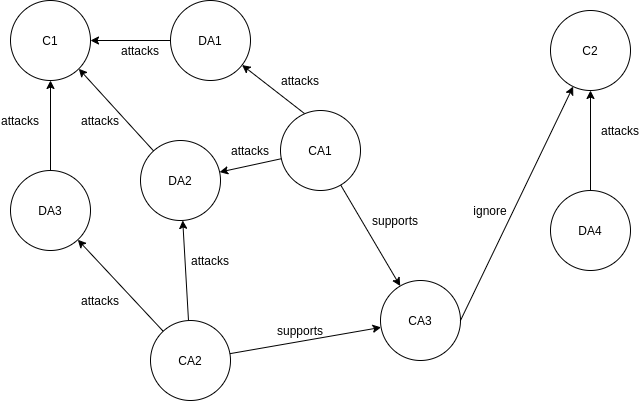
\includegraphics[width=5in]{figures/arguments.png}
  \caption[Arguments for claim 1]{\small arguments}
  \label{fig:monitoring-test}
\end{figure}

\subsection{Conclusions}

The proximate cause was found to be a war risk since the actions of the crew nor the Dominican government forced the actions of the rebels or the American forces.

Further, since the term 'requisition' is ambiguous, it is interpreted in favour of the plaintiff and the loss is determined not to fall under the exceptions of the War Risk Policy. 

\FloatBarrier
